

%----------------------------------------------------------------------------------------
%	PACKAGES AND OTHER DOCUMENT CONFIGURATIONS
%----------------------------------------------------------------------------------------

\documentclass[12pt]{article}

\usepackage{polski}
\usepackage[polish]{babel}
\usepackage[utf8]{inputenc} 
\usepackage{datetime}
\usepackage{graphicx}
\usepackage{tikz}
\usepackage{amsmath}
\usepackage{epstopdf}
\usepackage{multirow}
\usepackage{tabularx}
%\usepackage[colorlinks=true]{hyperref}
%\usepackage[all]{hypcap}
%\usepackage{showframe} 
\usepackage{geometry}
 \geometry{
 a4paper, 
 left=20mm,
 right=20mm,
 top=20mm,
 bottom=20mm,
 }
 
\renewcommand{\dateseparator}{.}
\newdate{exercise_date}{01}{04}{2014}
\newdate{create_date}{08}{04}{2014}

%----------------------------------------------------------------------------------------

%----------------------------------------------------------------------------------------
% TIKZ PACKAGES
%----------------------------------------------------------------------------------------
 
\usetikzlibrary{arrows, decorations.markings, decorations.pathmorphing, calc,
positioning}

%----------------------------------------------------------------------------------------

\begin{document}

\begin{titlepage}

\newcommand{\HRule}{\rule{\linewidth}{0.5mm}}
% Defines a new command for the horizontal lines, change thickness here

\center
% Center everything on the page
 
%----------------------------------------------------------------------------------------
%	LOGO SECTION
%----------------------------------------------------------------------------------------


\includegraphics[width=6cm]{../res/img/logo.png}\\[1cm]
% Include a department/university logo - this will require the graphicx package
 
%----------------------------------------------------------------------------------------
 
%----------------------------------------------------------------------------------------
%	HEADING SECTIONS
%----------------------------------------------------------------------------------------

\textsc{\LARGE Akademia Górniczo-Hutnicza \\[0.2cm]
im. Stanisława Staszica w Krakowie}\\[1.5cm]
% Name of your university/college

\textsc{\Large Podstawy Automatyki}\\[0.5cm]
% Major heading such as course name

%----------------------------------------------------------------------------------------
%	TITLE SECTION
%----------------------------------------------------------------------------------------

\HRule \\[0.5cm]
{ \huge \bfseries Dyskretne układy regulacji \\[0.3cm] oraz \\[0.5cm] Analiza
serwomechanizmu \\[0.2cm] przekaźnikowego z wykorzystaniem płaszczyzny
fazowej}\\[0.3cm]
% Title of your document
\HRule \\[1.5cm]
 
%----------------------------------------------------------------------------------------
%	AUTHOR SECTION
%----------------------------------------------------------------------------------------

% \begin{minipage}{0.4\textwidth}
% \begin{flushleft} \large
% \emph{Author:}\\
% Konrad \textsc{Adasiewcz} % Your name
% \end{flushleft}
% \end{minipage}
% ~
% \begin{minipage}{0.4\textwidth}
% \begin{flushright} \large
% \emph{Supervisor:} \\
% dr inż. Paweł \textsc{Rotter} % Supervisor's Name
% \end{flushright}
% \end{minipage}\\[4cm]

% If you don't want a supervisor, uncomment the two lines below and remove the section above
\flushright
\Large \emph{Autorzy:}\\
Konrad \textsc{Adasiewcz}\\[0.1cm] % Your name
Michał \textsc{Maciejewski}\\[3cm] % Your name

%----------------------------------------------------------------------------------------
%	DATE SECTION
%----------------------------------------------------------------------------------------
Data wykonania ćwiczenia: \\
{\large \displaydate{exercise_date}}\\[1cm]


\vfill % Fill the rest of the page with whitespace

\end{titlepage}

\section{Wstęp}

\subsection{Cel ćwiczenia}

Celem ćwiczenia jest zapoznanie się z przykładowym oprogramowaniem pozwalającym
na realizację sterowania cyfrowego w oparciu o komputer klasy PC oraz
zapoznanie się z przykładem interfejsu procesowego dla komputera klasy PC. 

\subsection{Opis stanowiska} 
Stanowisko laboratoryjne składa się z komputera PC z zainstalowanym pakietem
\textsc{GENIE} oraz stacji akwizycji danych \textit{ADAM5000} wyposażonej w
odpowiednie moduły we/wy:

\begin{itemize}
  \item \textit{ADAM5060} - dyskretne wyjścia przekaźnikowe
  \item \textit{ADAM5018} - wejścia analogowe specjalizowane do obsługi termopar
  \item \textit{ADAM5013} - wejścia termometru oporowego \textsc{Pt100}
\end{itemize}

\begin{figure}[!htb]
	\begin{center}
		\begin{tikzpicture}
	\coordinate (BL) 	at 	(0,0);
	\coordinate (TR) 	at 	(10,5);
	\coordinate (BLR) 	at 	(3,-4);
	\coordinate (TRR) 	at 	(7,-1);
	\coordinate (HSH) 	at 	(4.5,1.5);
	
	\coordinate (PT1) 	at 	($(BL)+(5-0.3,0)$);
	\coordinate (PT2) 	at 	($(BL)+(5,0)$);
	\coordinate (PT3) 	at 	($(BL)+(5+0.3,0)$);
	\coordinate (W1) 	at 	($(TR)+(-1.5,-5)$);
	\coordinate (W2) 	at 	($(TR)+(-2,-5)$);
	\coordinate	(W0)	at	($(W2)+(0.25,2.5)$); 
	\coordinate (H1I)	at	($(BL)+(HSH)+(0,0.3)$);
	\coordinate (H2I)	at	($(BL)+(HSH)+(0,1.7)$);
	\coordinate (H1B)	at	($(BL)+(1.5,0)$);
	\coordinate (H2B)	at	($(BL)+(2,0)$);
	
	\path[name path=H1Ih] (H1I) -- ++(-4,0);
	\path[name path=H2Ih] (H2I) -- ++(-4,0);
	\path[name path=H1Bv] (H1B) -- ++(0,4);
	\path[name path=H2Bv] (H2B) -- ++(0,4);
	
	\path[name intersections={of=H1Ih and H2Bv}];
	\coordinate (H1IB) at (intersection-1);
	\path[name intersections={of=H2Ih and H1Bv}];
	\coordinate (H2IB) at (intersection-1);
	
	\draw
		(H1B)	--
		(H2IB)	--
		(H2I);
	\draw
		(H2B)	--
		(H1IB)	--
		(H1I);

	\draw
		(W2)
		++(-0.5,1.5)	rectangle
		++(1.5,2);
	\draw
		(W0) .. controls +(120:1) and +(60:1) .. (W0)
		(W0) .. controls +(-120:1) and +(-60:1) .. (W0)
		(W0) .. controls +(-30:1) and +(30:1) .. (W0)
		(W0) .. controls +(150:1) and +(-150:1) .. (W0);
	\draw[-latex]
		(W0)
		++(-1,0)	--
		+(-1,0);
	\draw[-latex]
		(W0)
		++(-1,0.5)	--
		+(-1,0); 
	\draw[-latex]
		(W0)
		++(-1,-0.5)	--
		+(-1,0);
	\draw
		(W0)	circle (0.7);
	\draw
		(W1)	--
		++(0,1.5)
		(W2)	--
		++(0,1.5);
		
	\draw
		(H1B)	--
		++(0,-1)
		+(0,-0.07)	circle (0.07)	node[left,yshift=-6]{$230V$}
		++(0,-0.5)	circle (0.07)
		++(0,-0.07)	--
		++(0,-1.25)	--
		+(1.5,0);
	\draw
		(H2B)		--
		++(0,-2.2)	--
		+(1,0)	node[right,yshift=-10]{\textsc{Wyj}};

	\draw
		(W1)	--
		++(0,-1)
		+(0,-0.07)	circle (0.07)	node[right,yshift=-6]{$230V$}
		++(0,-0.5)	circle (0.07)
		++(0,-0.07)	--
		++(0,-1.25)	--
		+(-1.5,0);
	\draw
		(W2)		--
		++(0,-2.2)	--
		+(-1,0)	node[left,yshift=-10]{\textsc{Al1}};
		
	\draw
		(BLR)	node[below right]{\textsc{RE31}}; 

	\draw
		(BLR)	rectangle
		(TRR);
		
	\draw
		(PT1)	--
		++(0,-1)
		(PT2)	--
		++(0,-1)	node[below]{\textsc{Wej}}
		(PT3)	--
		++(0,-1);

	\draw
		(H1I)			--
		++(0.3,0)		--
		++(0.4,1.4/6)	--
		++(-0.4,1.4/6)	--
		++(0.4,1.4/6)	--
		++(-0.4,1.4/6)	--
		++(0.4,1.4/6)	--
		++(-0.4,1.4/6)	--
		(H2I);
	
	\draw[dashed]
		(BL) rectangle (TR);
	\draw
		($(BL)+(HSH)$)	rectangle
		($(TR)-(HSH)$);
	\filldraw[color=black]
		(BL)
		++(5-0.3,0) circle 	(0.07)
		++(0.3,0) 	circle 	(0.07)
		++(0.3,0) 	circle 	(0.07);
	\filldraw[color=black]
		(TR)
		++(-5-0.3,0)circle 	(0.07)
		++(0.3,0) 	circle 	(0.07)
		++(0.3,0) 	circle 	(0.07);
	\filldraw[color=black]
		(W1)		circle 	(0.07)
		(W2)		circle 	(0.07);
	\filldraw[color=black]
		(H1B)		circle 	(0.07)
		(H2B)		circle 	(0.07);
		
	\draw	%PT1001
		($(BL)+(HSH)$)
		++(0.4,0)		rectangle
		++(0.2,-0.5)
		++(-0.1,0)		--
		++(0,-1)
		++(0,1)			--
		++(-0.3,-0.3)	--
		++(0,-0.7)
		++(0.3,1)		--	node[above right]{\textsc{\small Pt100}}
		++(0.3,-0.3)	--
		++(0,-0.7);
	\draw	%PT1002
		($(TR)-(HSH)$)
		++(-0.4,0)		rectangle
		++(-0.2,0.5)
		++(0.1,0)		--
		++(0,1)
		++(0,-1)		--	node[below right]{\textsc{\small Pt100}}
		++(0.3,0.3)		--
		++(0,0.7)
		++(-0.3,-1)		--
		++(-0.3,0.3)	--
		++(0,0.7);
	
\end{tikzpicture}
	\end{center}
	\caption{Schemat stanowiska}
\end{figure}

\newpage

\section{Przebieg ćwiczenia}

Ćwiczenie składa się z dwóch części:

\begin{itemize}
  \item Realizacja zmierzchowego włącznika oświetlenia
  \item Realizacja dwupołożeniowego regulatora temperatury
\end{itemize}

Po sprawdzeniu poprawności działania podstawowych funkcjonalności stanowiska
prostymi programami testowymi przystąpiliśmy do wykonania ćwiczenia.

\subsection{Włącznik zmierzchowy}

Zamierzona strategia działania włącznika jest następująca:

\begin{itemize}
  \item Włączenie lampy na pewien zadany czas, gdy poziom oświetlenia spadnie
  poniżej wartości progowej
  \item Możliwość niezależnego od czujnika stałego włączenia lampy
  \item Możliwość zablokowania automatu włączającego lampę
  \item Pomiar aktualnej temperatury czujnikiem rezystancyjnym \textsc{Pt100}
\end{itemize}

Dodatkowo w oknie \textit{Display} należy umieścić wizualizację czasowego
przebiegu aktualnego oświetlenia i zadanego progu zadziałania, oraz aktualną
temperaturę otoczenia. Po krótkim przeanalizowaniu postawionego problemu
stworzyliśmy następujący schemat działania projektowanego włącznika:

\begin{figure}[!htb]
	\begin{center}
		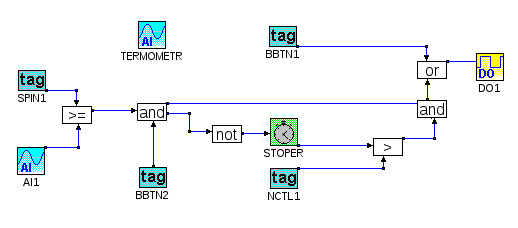
\includegraphics[width=\linewidth]{../res/img/task1.png}
	\end{center}
	\caption{Schemat włącznika zmierzchowego}\label{sch:task1}
\end{figure}

Funkcje logiczne sterujące stoperem i lampą to:

\begin{equation*}
	DO1=ON/OFF\vee ((STOPER\leq CZAS)\wedge \overline{BLOCK}\wedge (POZIOM\leq
	PROG))
\end{equation*}

\begin{equation*}
	STOPER\_RST=\overline{\overline{BLOCK}\wedge (POZIOM\leq PROG)}
\end{equation*}

\newpage

\begin{figure}[!htb]
	\begin{center}
		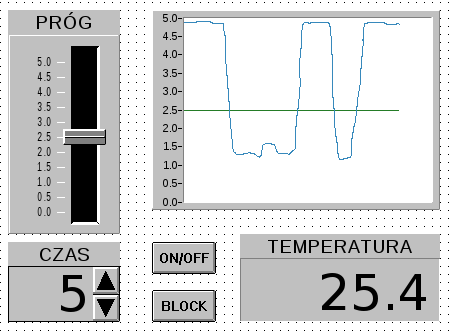
\includegraphics[width=\linewidth]{../res/img/disp1.png}
	\end{center}
	\caption{Wizualizacja działania włącznika zmierzchowego}
\end{figure} 

Na panelu operatorskim zostały umieszczone kontrolki zawarte w opisie wykonania
zadania.

W trakcie trwania ćwiczenia w celu sprawdzenia poprawności działania
zaprojektowanego włącznika został sprawdzony szereg scenariuszy przebiegu
natężenia oświetlenia i w każdym wypadku włącznik działał zgodnie z założonymi
wytycznymi.

Opis poszczególnych bloków na schemacie \ref{sch:task1}:

\begin{itemize}
  \item AI1 - wejście ogniwa fotowoltaicznego
  \item DO1 - przekaźnik załączający lampę
  \item BBINT1 - przycisk ON/OFF niezależnie włączający lampę
  \item BBINT2 - przycisk BLOCK blokujący automat załączający lampę
  \item NCTL1 - formant w którym w oknie display wybieramy czas świecenia lampy
  \item SPIN1 - formant w którym w oknie display wybieramy próg zadziałania
  włącznika
\end{itemize}

\newpage

\subsection{Dwupołożeniowy regulator temperatury}

Drugą częścią ćwiczenia jest implementacja dwupołożeniowego regulatora
temperatury, gdzie elementem grzewczym będzie lampa, natomiast obiektem
regulacji i jednocześnie czujnikiem pomiarowym jest czujnik \textsc{Pt100}
podłączony do modułu \textit{ADAM5013}.

Do jego realizacji użyliśmy wbudowanego w pakiet \textsc{GENIE} bloku
\textit{ON/OFF}. Blok ten posiada dwa wejścia, ustalające wartość zadaną oraz
wejście przyjmujące sygnał regulowany, i jedno wyjście załączające element
wykonawczy. Histerezę regulacyjną ustawia się wewnątrz bloku \textit{ON/OFF}. W
zaprezentowanym przykładzie histereza wynosi $\pm 1^{\circ}C$

\begin{figure}[!htb]
	\begin{center}
		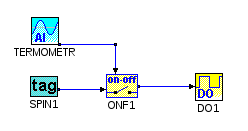
\includegraphics[width=9cm]{../res/img/task2.png}
	\end{center}
	\caption{Schemat układu regulacji}
\end{figure}

\begin{figure}[!htb]
	\begin{center}
		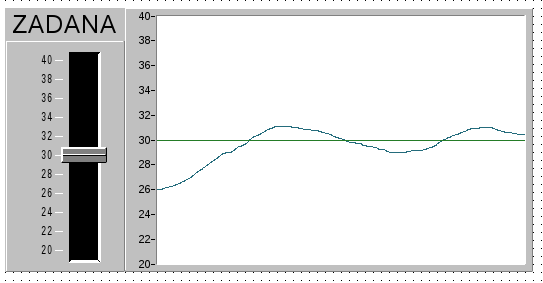
\includegraphics[width=\linewidth]{../res/img/disp2.png}
	\end{center}
	\caption{Wizualizacja działania regulatora}
\end{figure} 

\newpage

\section{Wnioski i spostrzeżenia}

W ćwiczeniu zapoznaliśmy się z działaniem systemu akwizycji danych opartym na
stacji firmy \textsc{Advantech}. Z jego pomocą jesteśmy w stanie zaimplementować
algorytmy sterowania procesami, oraz utworzyć prosty panel operatorski z
możliwością zadania nastaw i obserwacji wyników działania w czasie prawie
rzeczywistym.
Producent przewidział rozszerzenie podstawowej funkcjonalności stacji
\textit{ADAM} przez szereg dołączalnych modułów, dzięki którym jesteśmy w stanie
sterować elementami wykonawczymi, dokonać pomiaru napięcia analogowego, czy w
sposób uproszczony do minimum odczytywać temperaturę z zewnętrznych czujników
rezystancyjnych tudzież termoparowych.

Obydwa zadania postawione w instrukcji były na tyle nieskomplikowane, iż byliśmy
w stanie zaimplementować je ograniczając się do użycia standardowych bloków
pakietu \textsc{GENIE}.

\end{document}


